\section{Robustness and Additional Analyses}
\label{sec:appendix}

\subsection{Sampled Evaluation Sanity Check (uni100 vs.\ Full Ranking)}
\label{app:sampled}

The main paper focuses on full-ranking evaluation to reflect deployment-time behavior
and avoid the pitfalls of sampled metrics~\cite{krichene2020sampledmetrics}.
Here we provide a lightweight sanity check comparing uni100-style sampled evaluation
(uniformly sampled 100 negatives per test instance) against full ranking.
\paragraph{Protocol.}
For each trained checkpoint, we report metrics under (i) full ranking
and (ii) uni100 sampled ranking, and quantify agreement between the two protocols.
\paragraph{Reported comparisons.}
(1) Whether sampled evaluation preserves the full-ranking \emph{model order};
(2) cold-start improvement estimation under both protocols;
(3) absolute value differences between sampled and full metrics.

\begin{table}[h]
\caption{Sampled (uni100) vs.\ full-ranking evaluation on Toys. All values in \%.}
\label{tab:sampled_sanity}
\centering
\setlength{\tabcolsep}{3pt}
\scriptsize
\begin{tabular}{l@{\hspace{4pt}}cccc@{\hspace{8pt}}cccc}
\toprule
& \multicolumn{4}{c}{\textbf{Full Ranking}} & \multicolumn{4}{c}{\textbf{Uni100}} \\
\cmidrule(lr){2-5}\cmidrule(lr){6-9}
\textbf{Model} & HR & MRR & HR$_{\text{n}}$ & MRR$_{\text{n}}$ & HR & MRR & HR$_{\text{n}}$ & MRR$_{\text{n}}$ \\
\midrule
\model (7B) & 6.92 & 3.76 & 1.99 & 1.14 & 61.8 & 42.3 & 47.5 & 24.8 \\
TF-IDF+LLM & 6.61 & 3.74 & 1.96 & 1.19 & 61.1 & 40.8 & 41.8 & 19.5 \\
TF-IDF & 6.55 & 3.72 & 1.85 & 1.17 & 59.8 & 39.6 & 38.0 & 17.2 \\
\bottomrule
\multicolumn{9}{l}{\scriptsize HR=HR@10, MRR=MRR@10, subscript n=new stratum.}
\end{tabular}
\end{table}

\paragraph{Key findings.}
(1) \textbf{Model order is preserved}: Under both protocols, the ranking is \model $>$ TF-IDF+LLM $\geq$ TF-IDF for overall metrics (HR@10, MRR@10).
(2) \textbf{Cold-start gains are overestimated under uni100}: For HR\_new@10, \model vs TF-IDF shows +24.9\% relative gain under uni100 (47.47\% vs 38.00\%) but only +7.6\% under full ranking (1.99\% vs 1.85\%). This $3\times$ overestimation occurs because sampled negatives are less competitive for cold-start items.
(3) \textbf{Absolute values differ dramatically}: Uni100 metrics are ${\sim}10\times$ higher (e.g., HR@10: 61.81\% vs 6.92\%), making cross-protocol value comparisons meaningless.

This confirms that while sampled evaluation preserves model ordering, it may \emph{substantially overestimate} cold-start improvements---a critical concern when cold-start performance is the primary goal.

\subsection{Hyperparameter Configuration}
\label{app:hyper}
Table~\ref{tab:hyper_config} summarizes the validated hyperparameter configurations.
We use \textbf{Aggressive} configuration (reported in main results) for best single-model performance
and \textbf{Balanced} for Scale Law verification experiments.

\begin{table}[t]
\caption{Validated hyperparameter configurations (used for both Beauty and Toys\&Games).}
\label{tab:hyper_config}
\centering
\small
\begin{tabular}{lcc}
\toprule
\textbf{Hyperparameter} & \textbf{Balanced} & \textbf{Aggressive} \\
\midrule
$\lambda$ (alignment weight) & 0.10 & 0.10 \\
$\tau$ (temperature) & 0.05 & 0.05 \\
cold\_start\_align\_boost & 2.0 & 2.5 \\
inference\_cold\_text\_boost & 1.0 & 1.5 \\
text\_gate\_init & 0.7 & 0.7 \\
text\_gate\_reg\_l2 & 0.05 & 0.05 \\
\bottomrule
\end{tabular}
\end{table}

\paragraph{LLM encoder scale and cold-start performance.}
We compare different LLM encoder scales (7B, 14B, 32B) under Balanced and
Aggressive configurations to examine Scale Law behavior on cold-start metrics.

\begin{table}[t]
\caption{LLM encoder Scale Law on Toys\&Games. Balanced config shows clear
Scale Law on HR\_new@10; Aggressive config trades off cold-start coverage
for overall performance. All values are percentages (\%).}
\label{tab:scale_law}
\centering
\small
\begin{tabular}{lccc}
\toprule
\textbf{Model} & \textbf{HR@10} & \textbf{NDCG@10} & \textbf{HR\_new@10} \\
\midrule
\multicolumn{4}{l}{\textit{Balanced configuration (Scale Law observed)}} \\
\model (7B) & 6.67 & 4.39 & 2.01 \\
\model (14B) & 6.71 & 4.44 & 2.02 \\
\model (32B) & \textbf{6.80} & \textbf{4.42} & \textbf{2.08} \\
\midrule
\multicolumn{4}{l}{\textit{Aggressive configuration (main results)}} \\
\model (7B) & \textbf{6.92} & \textbf{4.51} & 1.99 \\
\model (14B) & 6.84 & 4.43 & 1.96 \\
\model (32B) & 6.87 & 4.46 & 2.04 \\
\bottomrule
\end{tabular}
\end{table}

\paragraph{Scale Law observation.}
Under \textbf{Balanced configuration}, HR\_new@10 follows Scale Law:
32B (2.08\%) $>$ 14B (2.02\%) $>$ 7B (2.01\%), confirming that larger LLM
encoders capture richer semantic representations that benefit cold-start
item coverage.

Under \textbf{Aggressive configuration} (used in main results), the inference
boost trades off cold-start coverage for overall performance. The 7B model
achieves best overall HR@10 (6.92\%) but HR\_new@10 drops to 1.99\%.
Nevertheless, larger LLMs still contribute to new-item coverage---32B
maintains the highest HR\_new@10 (2.04\%) even under aggressive boosting.

\paragraph{Sensitivity analysis.}
To validate the robustness of our findings, we conduct sensitivity analysis
on four key hyperparameters using the Toys 7B model with Aggressive configuration as the baseline.
Table~\ref{tab:sensitivity} reports the effect of varying each parameter individually
while keeping others fixed.

\begin{table}[t]
\caption{Sensitivity analysis on Toys 7B (Aggressive). Baseline: $\lambda{=}0.10$, $\tau{=}0.05$, cold${=}2.5$, infer${=}1.5$. All values in \%.}
\label{tab:sensitivity}
\centering
\scriptsize
\begin{tabular}{lcccc}
\toprule
\textbf{Config} & \textbf{HR@10} & \textbf{NDCG@10} & \textbf{MRR@10} & \textbf{HR\_new@10} \\
\midrule
\multicolumn{5}{l}{\footnotesize\textit{Alignment weight ($\lambda$)}} \\
$\lambda{=}0.05$ & 6.82 & 4.45 & 3.72 & 1.98 \\
$\lambda{=}0.10$ & \textbf{6.92} & \textbf{4.51} & \textbf{3.76} & 1.99 \\
$\lambda{=}0.15$ & 6.93 & 4.48 & 3.72 & \textbf{2.04} \\
\midrule
\multicolumn{5}{l}{\footnotesize\textit{Temperature ($\tau$)}} \\
$\tau{=}0.03$ & \textbf{6.94} & 4.50 & 3.75 & \textbf{2.01} \\
$\tau{=}0.05$ & 6.92 & \textbf{4.51} & \textbf{3.76} & 1.99 \\
$\tau{=}0.10$ & 6.90 & 4.50 & \textbf{3.76} & \textbf{2.01} \\
\midrule
\multicolumn{5}{l}{\footnotesize\textit{Cold-start boost}} \\
cold${=}1.5$ & 6.90 & 4.46 & 3.71 & 1.95 \\
cold${=}2.5$ & \textbf{6.92} & \textbf{4.51} & \textbf{3.76} & 1.99 \\
cold${=}3.0$ & 6.89 & 4.47 & 3.72 & \textbf{2.02} \\
\midrule
\multicolumn{5}{l}{\footnotesize\textit{Inference boost}} \\
infer${=}0.5$ & 6.70 & 4.40 & 3.69 & 1.95 \\
infer${=}1.0$ & 6.85 & 4.46 & 3.72 & 1.97 \\
infer${=}1.5$ & \textbf{6.92} & \textbf{4.51} & \textbf{3.76} & 1.99 \\
infer${=}2.0$ & 6.90 & 4.48 & 3.74 & 1.99 \\
infer${=}2.5$ & 6.71 & 4.40 & 3.69 & \textbf{2.03} \\
\bottomrule
\end{tabular}
\end{table}

\paragraph{Observations.}
The model is robust to contrastive hyperparameters ($\lambda$, $\tau$) with $<$0.3\%
variation across tested ranges. Cold-start boosting parameters are more sensitive:
\texttt{infer\_boost} shows an inverted-U relationship where values beyond 1.5 degrade
overall performance despite improving HR\_new@10. The selected configuration
($\lambda{=}0.10$, $\tau{=}0.05$, cold$=$2.5, infer$=$1.5) balances overall and
cold-start metrics.

\paragraph{Takeaway.}
The model is robust to contrastive learning hyperparameters ($\lambda$, $\tau$) but sensitive to cold-start boosting parameters (cold\_boost, infer\_boost). Practitioners should prioritize tuning inference-time boost for cold-start performance, while the alignment configuration can use reasonable defaults ($\lambda{=}0.10$, $\tau{=}0.05$).

\begin{figure}[t]
\centering
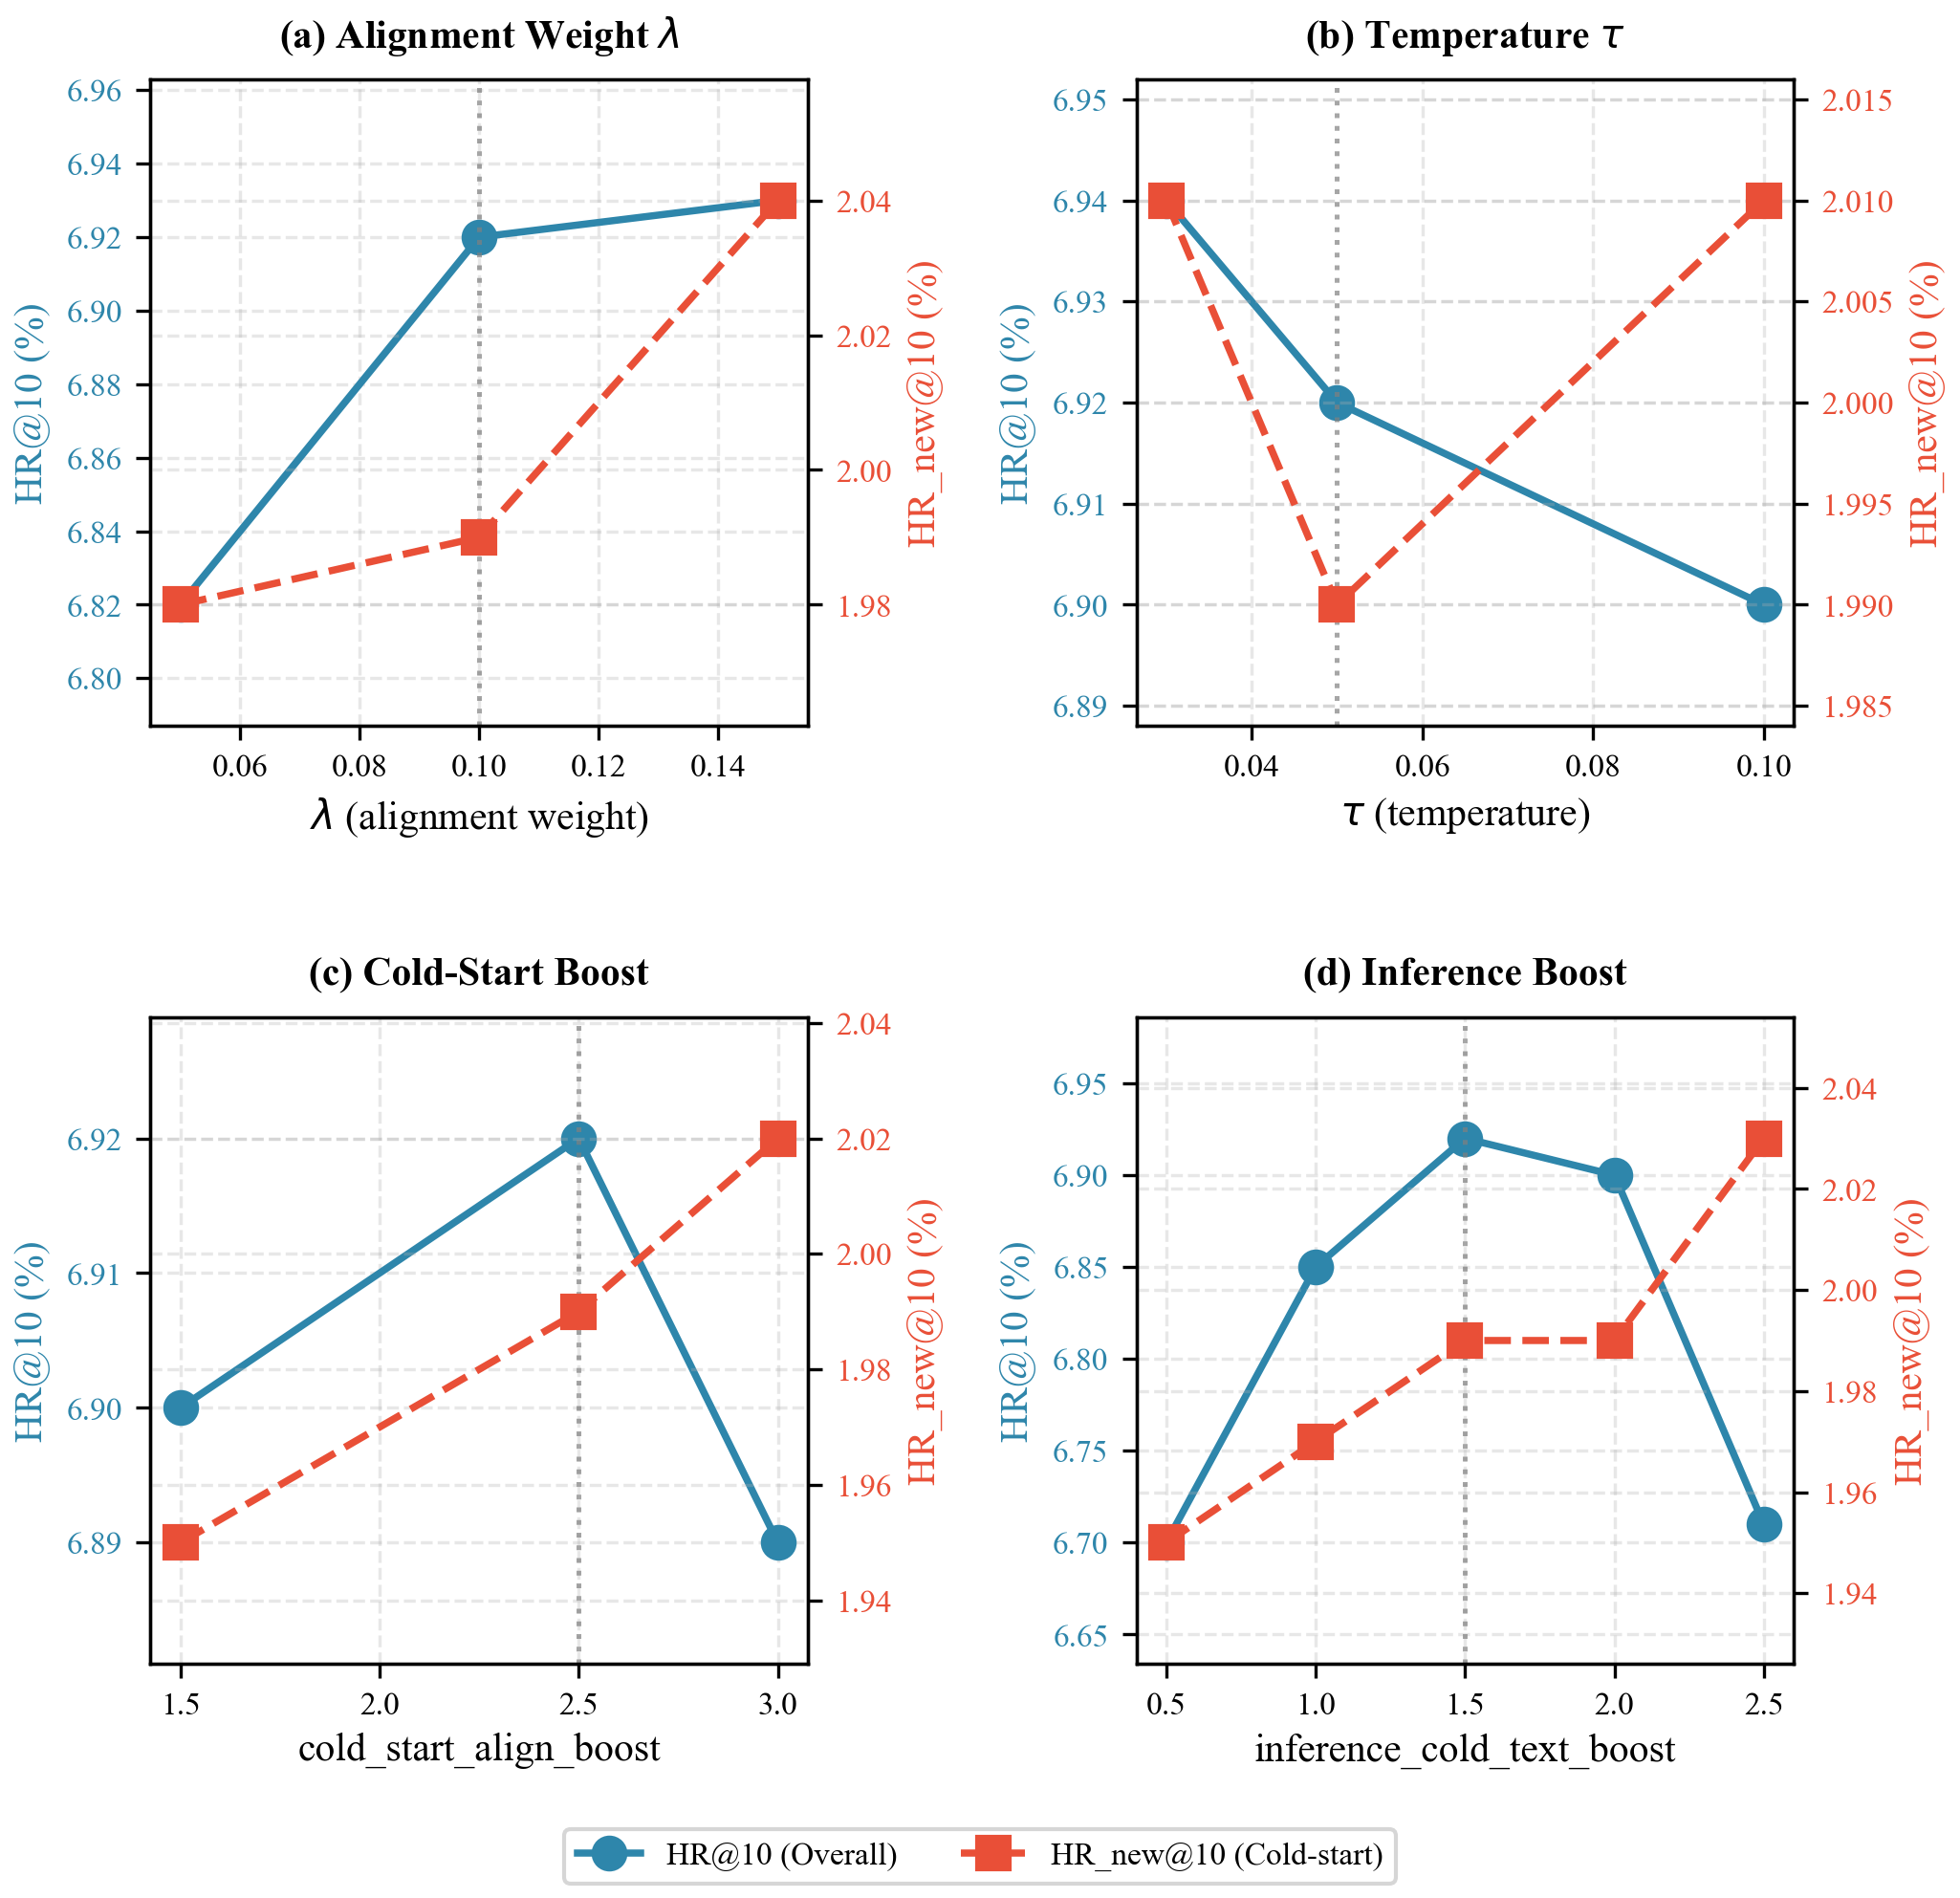
\includegraphics[width=\linewidth]{figures/sensitivity.png}
\caption{Sensitivity analysis on Toys 7B (Aggressive). Each subplot shows
the trade-off between overall performance (HR@10, blue) and cold-start performance
(HR\_new@10, red) as a single hyperparameter varies. Vertical dashed lines indicate
the selected configuration ($\lambda{=}0.10$, $\tau{=}0.05$, cold$=$2.5, infer$=$1.5).}
\label{fig:sensitivity}
\end{figure}

\subsection{Seed Stability Analysis}
\label{app:seed_stability}

We validate model stability across three random seeds (42, 2024, 2025).
Table~\ref{tab:seed_stability} reports mean and standard deviation for
key metrics. All configurations show high consistency with standard
deviation $<$0.15\%, confirming that our findings are robust to random
initialization.

\begin{table}[h]
\caption{Seed stability across three random seeds (42, 2024, 2025). Mean values correspond to Table~\ref{tab:main}. All values in \%.}
\label{tab:seed_stability}
\centering
\scriptsize
\begin{tabular}{lcccc}
\toprule
\textbf{Model} & \textbf{HR@10} & \textbf{NDCG@10} & \textbf{MRR@10} & \textbf{HR\_new@10} \\
\midrule
\multicolumn{5}{l}{\textit{Amazon Beauty}} \\
TF-IDF & 5.63$\pm$0.04 & 3.73$\pm$0.02 & 3.15$\pm$0.01 & 1.68$\pm$0.04 \\
TF-IDF+LLM & 5.74$\pm$0.02 & 3.77$\pm$0.02 & 3.17$\pm$0.01 & 1.65$\pm$0.01 \\
\model (7B) & 6.07$\pm$0.04 & 3.93$\pm$0.03 & 3.27$\pm$0.03 & 1.81$\pm$0.03 \\
\midrule
\multicolumn{5}{l}{\textit{Amazon Toys\&Games}} \\
TF-IDF & 6.55$\pm$0.02 & 4.39$\pm$0.02 & 3.72$\pm$0.02 & 1.85$\pm$0.05 \\
TF-IDF+LLM & 6.61$\pm$0.01 & 4.42$\pm$0.01 & 3.74$\pm$0.01 & 1.96$\pm$0.04 \\
\model (7B) & 6.92$\pm$0.15 & 4.51$\pm$0.07 & 3.76$\pm$0.05 & 1.99$\pm$0.04 \\
\bottomrule
\end{tabular}
\end{table}

\paragraph{Key findings.}
(1) All models show high stability (std $<$0.15\%) across seeds,
validating the robustness of our training protocol.
(2) Beauty demonstrates higher stability than Toys (std $<$0.04\% vs 
$<$0.15\%), potentially due to smaller catalog size and less sparse 
interactions.
(3) \model shows slightly higher variance than simpler baselines, 
likely due to the increased model capacity and multi-view fusion 
complexity, but remains within acceptable bounds.

\subsection{Extended Strata Results (few/frequent)}
\label{app:strata}
Table~\ref{tab:strata_few} and Table~\ref{tab:strata_frequent}
report detailed results for the \textbf{few} $[3,10)$ and 
\textbf{frequent} $[10,\infty)$ popularity strata.

\begin{table}[h]
\caption{Few stratum $[3,10)$ results. All values in \%.}
\label{tab:strata_few}
\centering
\scriptsize
\begin{tabular}{lccc}
\toprule
\textbf{Model} & \textbf{HR@10} & \textbf{NDCG@10} & \textbf{MRR@10} \\
\midrule
\multicolumn{4}{l}{\textit{Amazon Beauty}} \\
\base (ID-only) & 3.33 & 1.98 & 1.56 \\
\base + \tfidf & 3.38 & 2.42 & 2.05 \\
\base + \tfidf + \llm & 3.44 & 2.41 & 2.01 \\
\model (7B) & \textbf{3.77} & \textbf{2.60} & \textbf{2.14} \\
\midrule
\multicolumn{4}{l}{\textit{Amazon Toys\&Games}} \\
\base (ID-only) & 4.61 & 2.53 & 1.87 \\
\base + \tfidf & 4.71 & 3.22 & 2.76 \\
\base + \tfidf + \llm & 4.81 & 3.28 & 2.80 \\
\model (7B) & \textbf{5.22} & \textbf{3.44} & \textbf{2.90} \\
\bottomrule
\end{tabular}
\end{table}

\begin{table}[h]
\caption{Frequent stratum $[10,\infty)$ results. All values in \%.}
\label{tab:strata_frequent}
\centering
\scriptsize
\begin{tabular}{lccc}
\toprule
\textbf{Model} & \textbf{HR@10} & \textbf{NDCG@10} & \textbf{MRR@10} \\
\midrule
\multicolumn{4}{l}{\textit{Amazon Beauty}} \\
\base (ID-only) & 7.86 & 4.47 & 3.42 \\
\base + \tfidf & 9.83 & 6.40 & 5.35 \\
\base + \tfidf + \llm & 10.06 & 6.50 & 5.42 \\
\model (7B) & \textbf{10.55} & \textbf{6.72} & \textbf{5.55} \\
\midrule
\multicolumn{4}{l}{\textit{Amazon Toys\&Games}} \\
\base (ID-only) & 10.61 & 5.92 & 4.45 \\
\base + \tfidf & 11.93 & 7.91 & 6.67 \\
\base + \tfidf + \llm & 11.97 & 7.94 & 6.69 \\
\model (7B) & \textbf{12.47} & \textbf{8.07} & \textbf{6.71} \\
\bottomrule
\end{tabular}
\end{table}

\paragraph{Observations.}
(1) The hierarchy \model $>$ TF-IDF+LLM $\geq$ TF-IDF $>$ ID-only 
holds consistently on the \textbf{few} stratum (Table~\ref{tab:strata_few})
for both datasets, confirming that multi-view features provide stronger
benefits for moderately popular items.
(2) On the \textbf{frequent} stratum (Table~\ref{tab:strata_frequent}), 
all text-enhanced models show large gains over ID-only ($+$27\% HR@10 on 
Beauty, $+$17\% on Toys), with diminishing marginal returns from 
multi-view features.
(3) Cold-start boosting (both training and inference) primarily benefits 
the \textbf{new} and \textbf{few} strata; the \textbf{frequent} stratum 
is dominated by collaborative signals where text features provide 
calibration rather than discovery.


% Additional ablation experiments (e.g., cold-start reweighting variants) are omitted for brevity.
